\documentclass[11pt]{beamer}
\usepackage{verbatim}
\usepackage{amsmath}
\usepackage{amsthm}
\usepackage{graphics}
\usepackage{multicol}
\usepackage{color}
\usepackage{stmaryrd}\usefonttheme[onlymath]{serif}

\title{Progess Report 2}
\date{\today}
\author{Xie Li}
\begin{document}
\maketitle

\begin{frame}\frametitle{Overview of the Progress}
\begin{itemize}
\item A closer look into the source code of \textsc{CPAChecker}.

\item Towards Practical Predicate Analysis
\item Investigation of algorithm ABE (Adjust-Block Encoding).

\end{itemize}

\end{frame}

\begin{frame}\frametitle{Architecture of CPAChecker}
\begin{center}
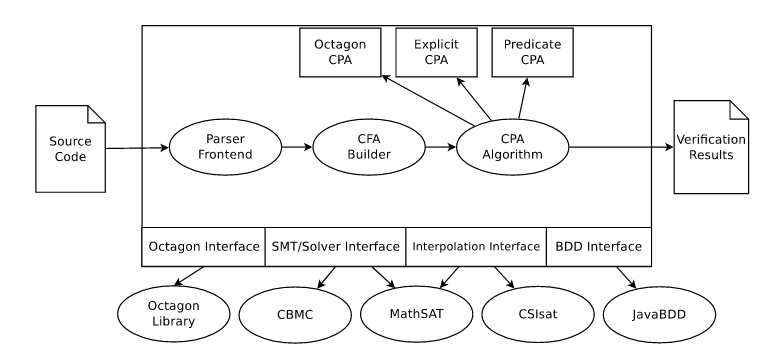
\includegraphics[scale=0.4]{cpa_arch.png}
\end{center}
The tool is developed in JAVA.
\end{frame}

\begin{frame}\frametitle{Parser Frontend}
The function of Parser Frontend module is converting the C, java or llvm IR into data structure CFA.

\begin{itemize}
\item C and JAVA: use toolchain in the eclipse CDT to parse the src code into AST and then convert to nodes of CFA.
\item LLVM: use their own developed package for llvm parsing.
\end{itemize}
\end{frame}

\begin{frame}\frametitle{Data Structures}
\begin{itemize}
\item CFA: is a interface which provides methods acquiring nodes, function heads, main function and information about loop structures.

CFA can be constructed using parsing results.


\item SpecificationProperty: a class giving entry of function, properties and specifications.
\begin{multicols}{2}
\begin{center}
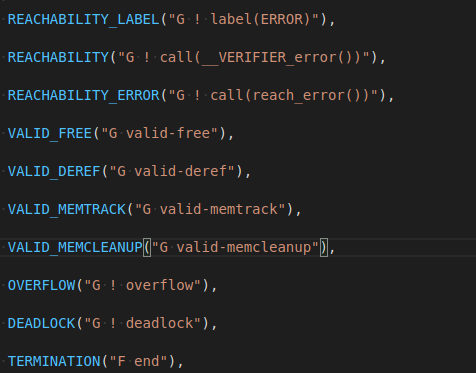
\includegraphics[scale=0.35]{commonP.png}

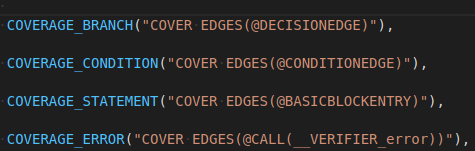
\includegraphics[scale=0.35]{commonC.png}
\end{center}
\end{multicols}

\end{itemize}

\end{frame}


\begin{frame}\frametitle{Algorithm}
The entry of the algorithm is in file CPAChecker.java where CPAChecker use factory to create different algorithm instances based on configurations fed to the program.

\begin{itemize}
\item CPA Algorithm.

\item Predicate Abstraction.

\item CEGAR.

\item Adjustable-Block Encoding...
\end{itemize}
\end{frame}
\begin{frame}\frametitle{CPA}
\begin{center}
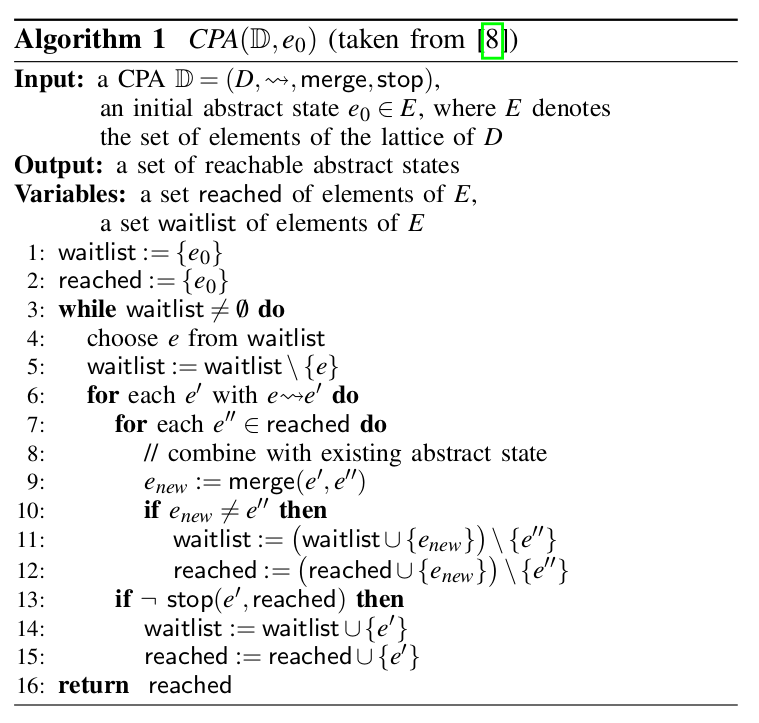
\includegraphics[scale=0.34]{cpa.png}
\end{center}
\end{frame}


\begin{frame}\frametitle{ABE}
\begin{center}
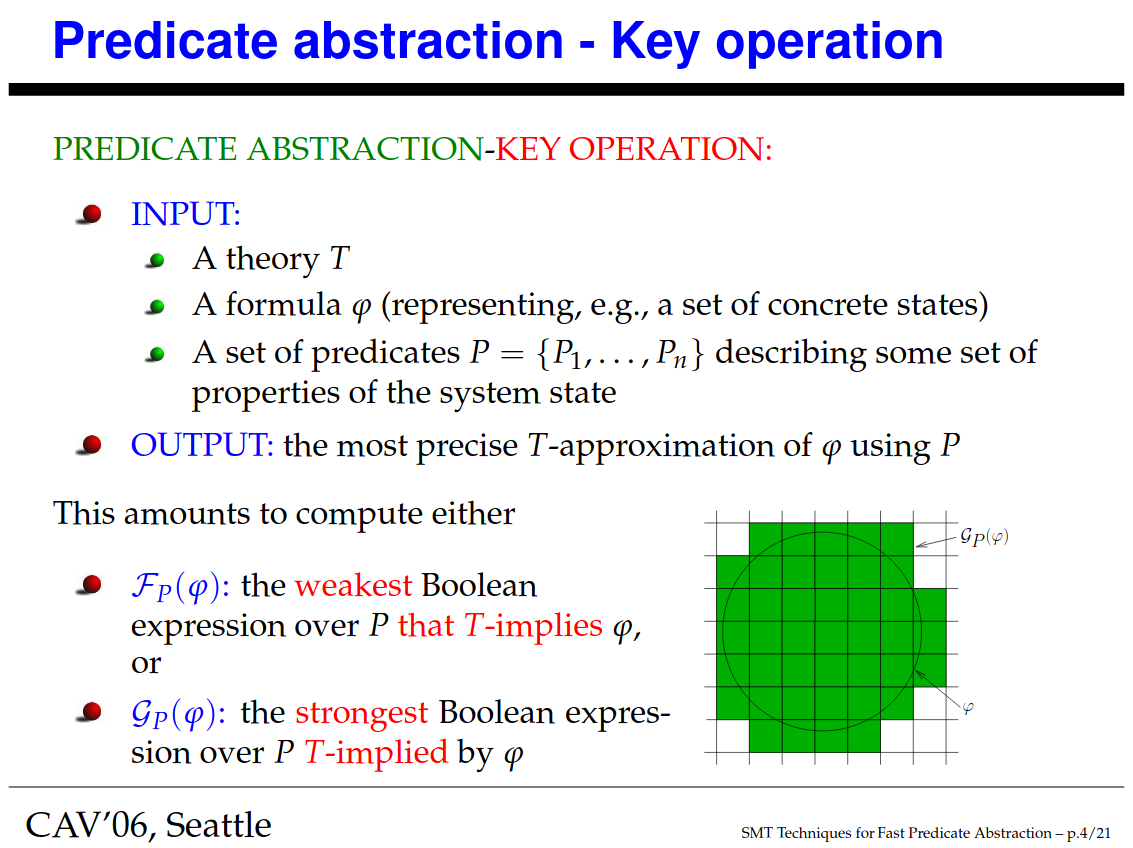
\includegraphics[scale=0.27]{pa.png}
\end{center}
\end{frame}

\begin{frame}\frametitle{ABE Example}

\begin{center}
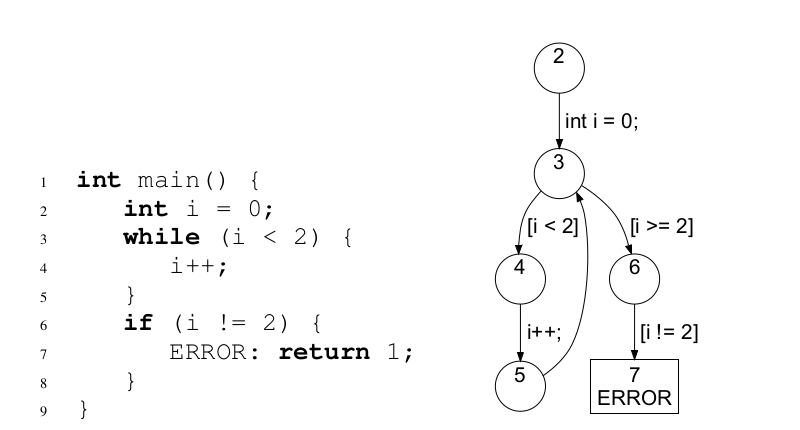
\includegraphics[scale=0.36]{cfa.png}
\end{center}

\end{frame}

\begin{frame}\frametitle{ABE example}
\begin{center}
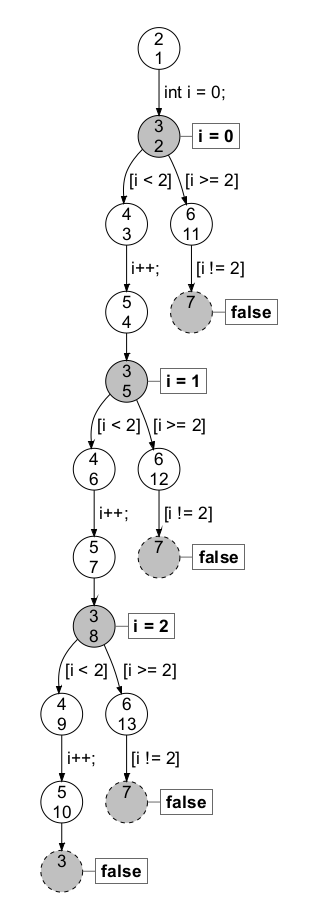
\includegraphics[scale=0.26]{a.png}
\end{center}
\end{frame}


\end{document}